\section{Introduction}

%%% INTRODUCTION AND SCOPE %%%%
Compositional and systematic generalization are core principles of human cognition \cite{fodor1988connectionism}. From a few examples of `atomic' concepts, humans can later effortlessly combine these in exponentially many new ways and apply them in contexts far removed from those in which they were learned. As Lake and Baroni illustrate, ``Once a person learns the meaning of a new verb ‘dax,’ they can immediately understand the meaning of ‘dax twice’ or ‘sing and dax’'' \cite{SCAN_lake_baroni}. Machine learning systems still struggle with these forms of generalization, making them a central research challenge \cite{galke2024deep, besold2016generality, wiedemer2023compositional, lake_baroni_2023, keysers2019measuring, xu2022compositional, wiedemer2023provable, brady2023provably}.

%%% WHAT PEOPLE DID ABOUT THE PROBLEM - & THE GAP WHICH WE EXPLOIT %%%
To foster progress in this direction, several benchmarks have been proposed, both in language \cite{SCAN_lake_baroni, schug2023discovering, keysers2019measuring, kim2020cogs, hupkes2020compositionality} and vision \cite{clevr, cvr2022, barrett2018measuring, fleuret2011comparing, mondorf2025enabling, girdhar2019cater}. Yet in vision, existing benchmarks lack the flexibility of their language counterparts: they provide limited control over compositional structure, offer a narrow range of tasks, and conflate visual complexity with relational structure -- distracting from the essence of compositional generalization.

%%% HOW WE CLOSE THE GAP %%%
To close this gap, we introduce \textbf{CO}mpositional \textbf{G}eneralization \textbf{I}n \textbf{T}ransformations \textbf{A}nd \textbf{O}bjects: \textbf{\generatorName} -- a procedural object-centric framework designed to generate simple, controllable datasets to probe compositional and systematic generalization in an abstract visual domain. Our generator's strength stems from its capacity to compose freely, at arbitrary compositional depth, a set of \ntransforms\ atomic transformations -- thus enabling to create millions of unique transformation sequences, with a virtually infinite amount of task samples, across a wide range of difficulties. 

In our \generatorName\ framework, models can learn to apply a given sequence of object-transformations and generate an `output grid' given an `input grid' and a transformation sequence (see Figure \ref{fig:task_examples}). Furthermore, models can be implemented in various environment configurations (e.g., with different numbers or types of objects, or grid dimensions). 

\begin{figure} [!htbp]
    \centering
    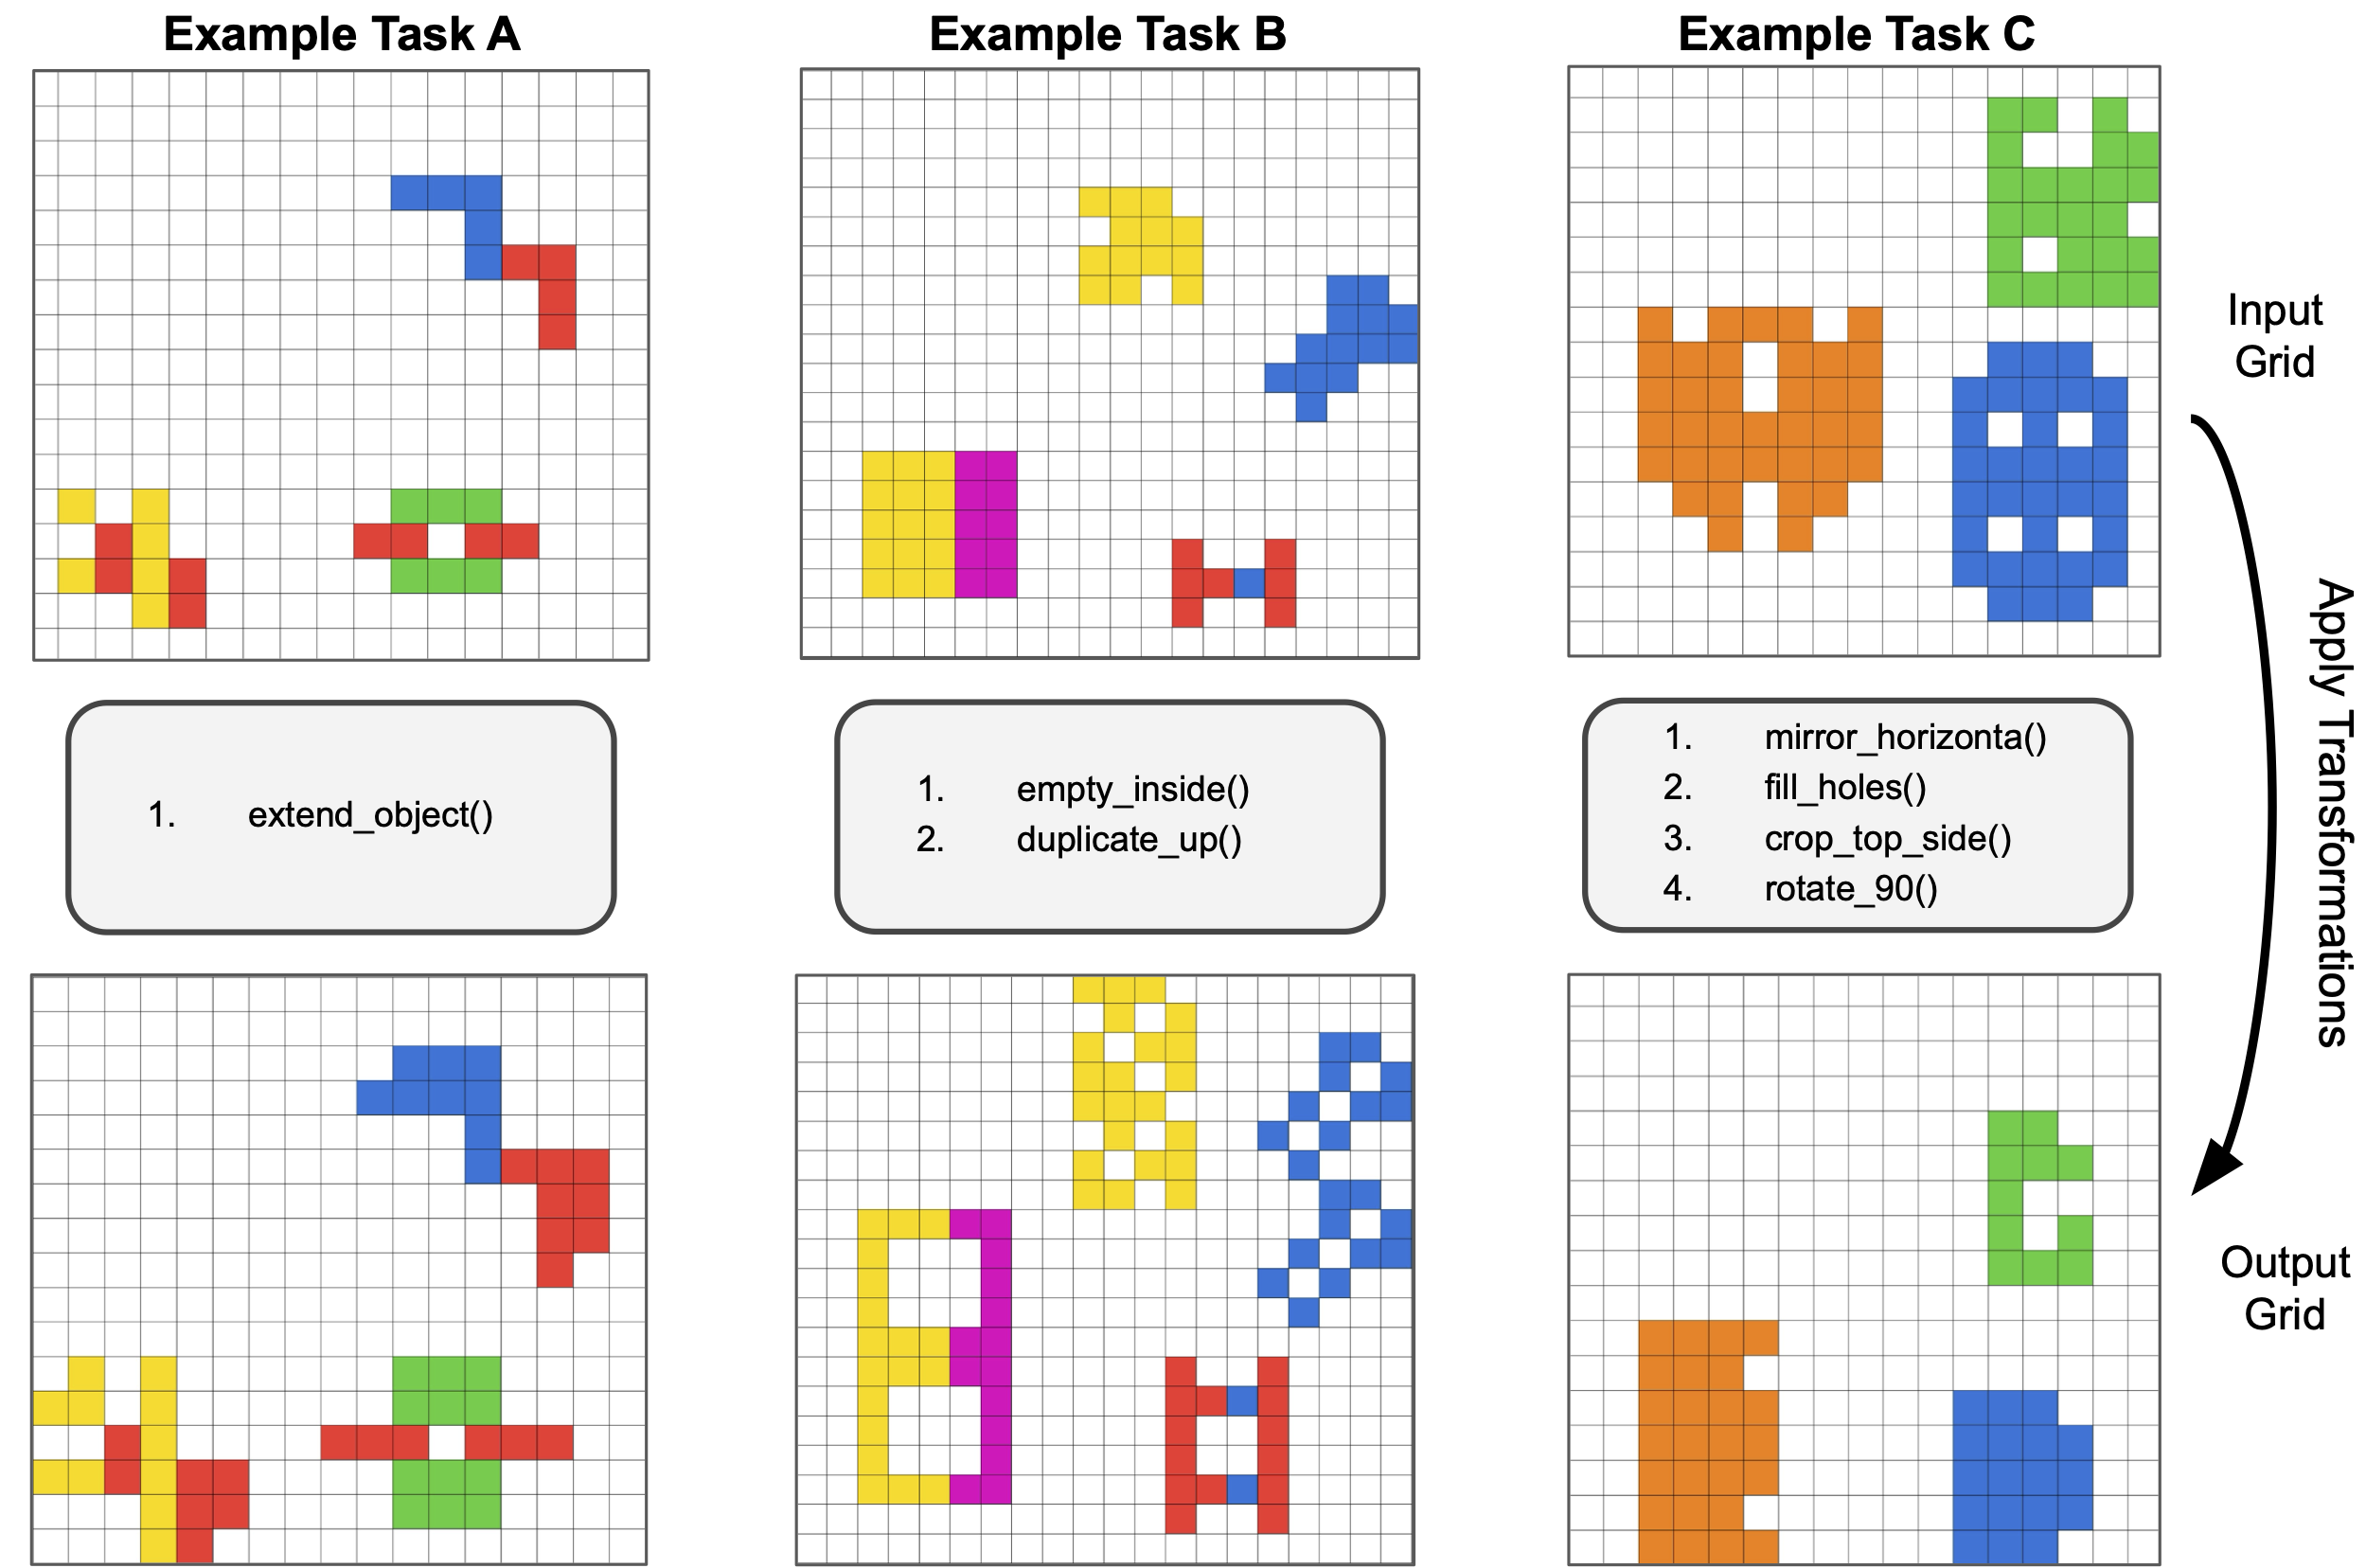
\includegraphics[width=0.95\columnwidth]{Figures/COGITAO_first_figure.png}
    \caption{Set of input-output pair examples from our \generatorName\ generator, with input grids on top rows, and corresponding output grids (after transforming input) on the bottom rows. Each input-output pair follows a different transformation sequence (see boxes on middle row) and a given grid/object parametrization.}
    \label{fig:task_examples}
\end{figure}

The key test of compositionality comes from varying transformation sequences and environment parameters between training and testing time. Analogous to the linguistic example ``dax twice'' or ``sing and dax'' \cite{SCAN_lake_baroni}, a model trained to ``rotate'' objects once should generalize to ``rotate twice'' or ``rotate and translate,'' provided it has seen the individual rotate and translate transformations during training.

%%% SOME CONTEXT ON THE CHOICES WE MAKE, OUR MOTIVATIONS AND LINKS TO OTHER LITERATURE%%%

\generatorName\ is deliberately abstract and synthetic, which enables to precisely isolate core compositional reasoning from confounding visual complexity. Despite its simplicity and grid-based nature, it captures compositional and systematic generalization in ways essential for real-world vision tasks. Indeed, the object-centric, order-dependent operations exemplified in \generatorName -- such as selectively modifying or relocating objects while preserving the surrounding scene -- mirror the challenges studied in robotics \cite{roy2004mental} and world-model research \cite{ha2018world, hafner2023masteringDREAMER, bruce2024GENIE, ferraro2025FOCUS}. We therefore position \generatorName\ not only as a static image benchmark, but also as an image-and-action framework that explicitly links perception to interaction (see Appendix \ref{appendix:sequential_COGITAO}). To facilitate transfer to natural vision, \generatorName\ additionally offers RGB renderings of its tasks to train standard computer-vision models (see Appendix \ref{appendix:rgb_cogitao}), while preserving all its diagnostic power.

%%% HOW WE EXEMPLIFY OUR BENCHMARK, AND WHAT MODELS WE LOOK AT FOR THAT %%%

To demonstrate our framework’s utility and support further research, we release a suite of benchmark datasets built from different \generatorName\ configurations. We train state-of-the-art architectures that incorporate inductive biases well suited for systematic and compositional generalization (Diffusion Transformers \cite{Nie_LLaDA_2025} and Pondering Looped Transformers \cite{banino2021pondernet, dehghani2019universaltransformers}). We also compare to baseline Transformers (optionally infused with object-centric inductive biases \cite{arc_vit} and ResNet \cite{he2015deepresiduallearningimage}. Our experiments intentionally target the raw inductive biases of well-specified architectures rather than large foundation models, whose training data and precise design details often remain opaque \footnote{We note that we also provide baseline foundation models results by adapting COGTIAO as an In-Context-Learning task for frontier LLMs, and highlight similar failure modes to models trained from scratch (see appendix \ref{appendix:llm_results})}. Despite solid in-domain performance, we report that these models consistently fail to generalize to novel combinations of familiar visual elements. Our findings highlight the need for architectures that move beyond pattern matching and memorization \cite{bahdanau2018systematic, geirhos2020shortcut, csordas2021devil, Faith_Fate} towards truly structured, compositional understanding -- \generatorName provides a simple framework to foster progress in this direction.

%%%% GOOD PARAGRAPH FROM RELATEDD WORKS TO ADD IF POSSIBLE  
% We are particularly interested in facilitating research into architectures and inductive biases that enable the emergence of compositional generalization (as opposed to forms of memorization \cite{bahdanau2018systematic, geirhos2020shortcut, csordas2021devil, Faith_Fate}) in an efficient and scalable way by training them with an appropriate amount of data from scratch. Hence, foundation models are considered out of the scope of this work.
%%%%
In this paper, our main contributions are:

\begin{enumerate}
    \item We introduce \generatorName: a procedural, grid-based and object-centric framework that freely composes 28 atomic object-transformations to generate millions of unique, controllable input–output rules at adjustable composition depth.
    \item We extend \generatorName\ beyond simple grids to RGB renderings for real-world vision transfer (see appendix \ref{appendix:rgb_cogitao}), and from single input–output pairs to sequences of images and actions for world-model research (see appendix \ref{appendix:sequential_COGITAO}).
    \item We create and release multiple benchmark datasets targeting specific aspects of compositional and systematic generalization, enabling reproducible and scalable experimentation.
    \item We provide cohesive baselines with state-of-the-art models known for their reasoning capabilities, and show that they consistently fail to generalize to out-of-distribution compositions --- highlighting the open challenge of systematic compositional generalization in object-centric domains. 
\end{enumerate}
